\documentclass[tikz,border=18pt]{standalone}
\usetikzlibrary{positioning,arrows.meta,fit,backgrounds,calc}

% ----- Diales rápidos -----
\def\colsep{74mm}   % separación horizontal entre columnas (núcleo <-> derecha/izquierda)
\def\midsep{18mm}   % separación a la columna INTERMEDIA (donde van 06 y 07)
\def\vsep{16mm}     % separación vertical entre cajas
\def\twcore{5.6cm}  % ancho de texto cajas núcleo
\def\twside{5.0cm}  % ancho de texto cajas laterales/intermedia

\begin{document}
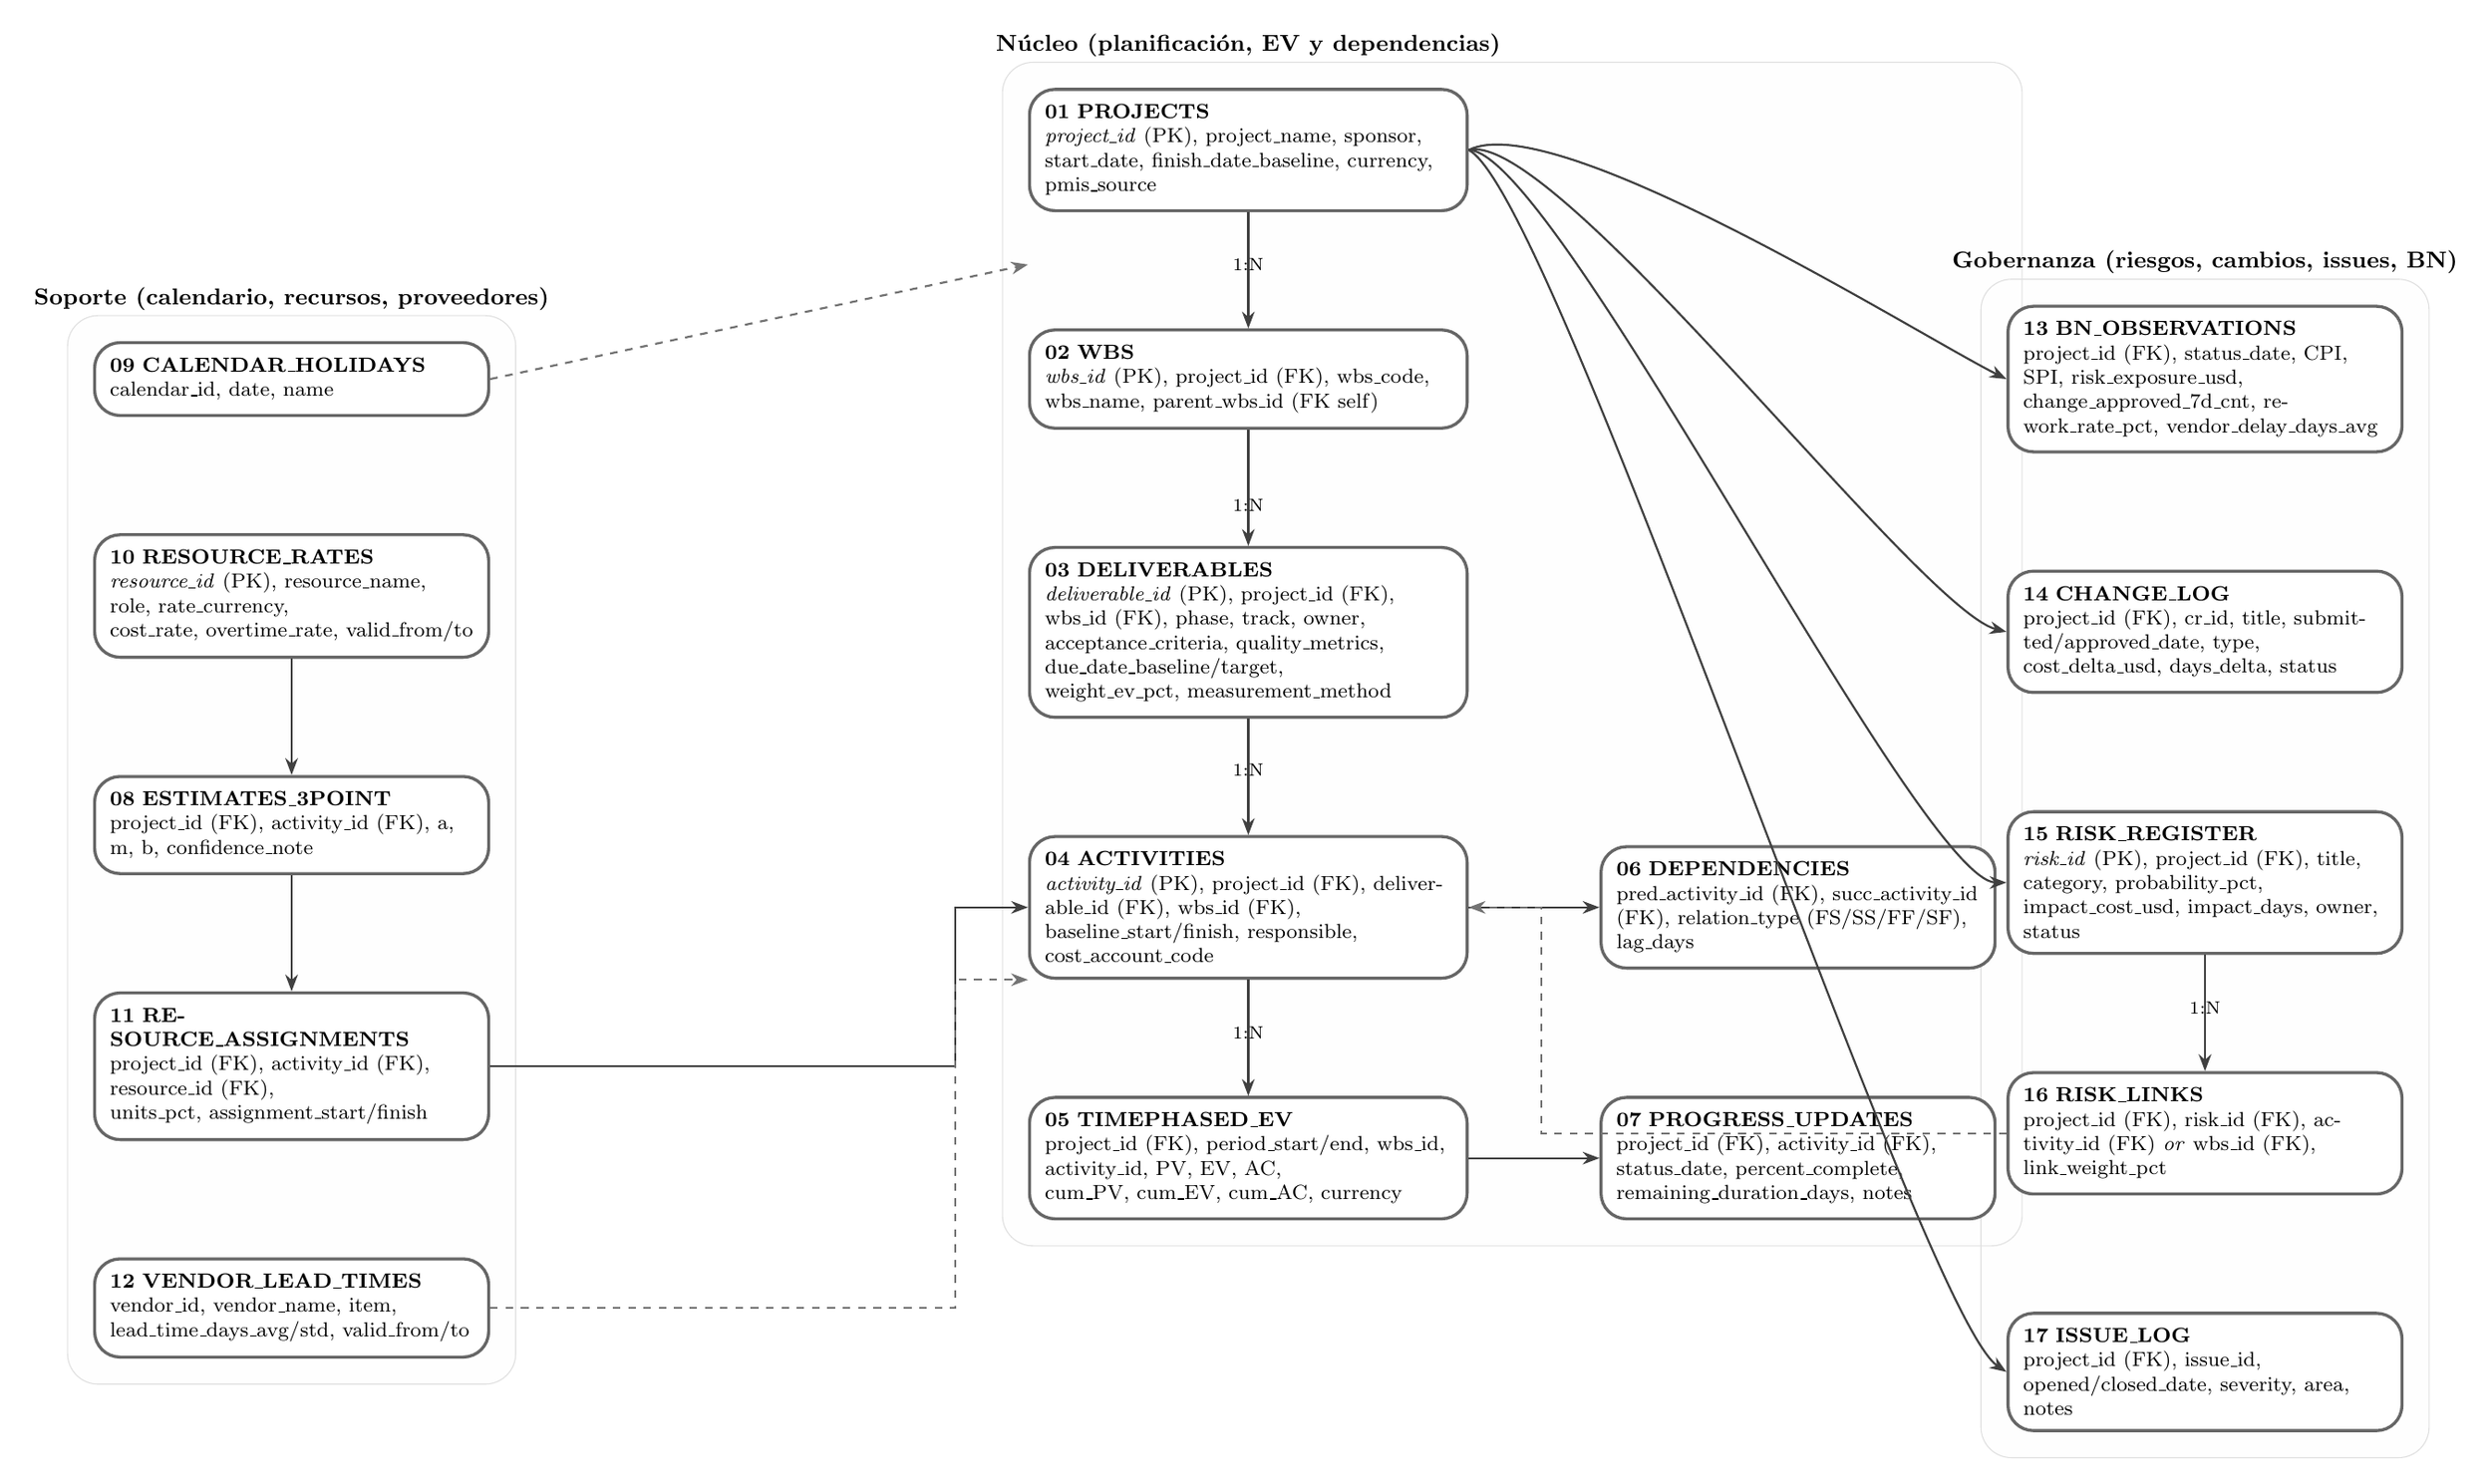
\begin{tikzpicture}[
  font=\footnotesize, % o \small si querés más grande
  entity/.style  = {rectangle, rounded corners=10pt, draw=black!60, very thick, fill=white,
                    text width=\twcore, align=left, inner sep=6pt},
  entityS/.style = {entity, text width=\twside},
  arr/.style     = {-{Stealth}, thick, draw=black!75},
  link/.style    = {-{Stealth}, thick, dashed, draw=black!55},
  zone/.style    = {rounded corners=12pt, fill=black!5, draw=black!12}
]

% ================== COLUMNA CENTRAL (NÚCLEO) ==================
\node (Project) [entity]
  {\textbf{01 PROJECTS}\\
   \emph{project\_id} (PK), project\_name, sponsor, start\_date, finish\_date\_baseline, currency, pmis\_source};

\node (WBS) [entity, below=\vsep of Project]
  {\textbf{02 WBS}\\
   \emph{wbs\_id} (PK), project\_id (FK), wbs\_code, wbs\_name, parent\_wbs\_id (FK self)};

\node (Deliv) [entity, below=\vsep of WBS]
  {\textbf{03 DELIVERABLES}\\
   \emph{deliverable\_id} (PK), project\_id (FK), wbs\_id (FK), phase, track, owner,\\
   acceptance\_criteria, quality\_metrics, due\_date\_baseline/target,\\
   weight\_ev\_pct, measurement\_method};

\node (Act) [entity, below=\vsep of Deliv]
  {\textbf{04 ACTIVITIES}\\
   \emph{activity\_id} (PK), project\_id (FK), deliverable\_id (FK), wbs\_id (FK),\\
   baseline\_start/finish, responsible, cost\_account\_code};

\node (TP) [entity, below=\vsep of Act]
  {\textbf{05 TIMEPHASED\_EV}\\
   project\_id (FK), period\_start/end, wbs\_id, activity\_id, PV, EV, AC,\\
   cum\_PV, cum\_EV, cum\_AC, currency};

% ===== COLUMNA INTERMEDIA (entre núcleo y derecha) =====
\node (Deps) [entityS, right=\midsep of Act]
  {\textbf{06 DEPENDENCIES}\\
   pred\_activity\_id (FK), succ\_activity\_id (FK), relation\_type (FS/SS/FF/SF), lag\_days};

\node (Prog) [entityS, right=\midsep of TP]
  {\textbf{07 PROGRESS\_UPDATES}\\
   project\_id (FK), activity\_id (FK), status\_date, percent\_complete,\\
   remaining\_duration\_days, notes};

% ================== COLUMNA IZQUIERDA (SOPORTE) ==================
\node (Cal)      [entityS, left=\colsep of WBS]
  {\textbf{09 CALENDAR\_HOLIDAYS}\\ calendar\_id, date, name};

\node (ResRates) [entityS, below=\vsep of Cal]
  {\textbf{10 RESOURCE\_RATES}\\
   \emph{resource\_id} (PK), resource\_name, role, rate\_currency,\\ cost\_rate, overtime\_rate, valid\_from/to};

\node (PERT)     [entityS, below=\vsep of ResRates]
  {\textbf{08 ESTIMATES\_3POINT}\\
   project\_id (FK), activity\_id (FK), a, m, b, confidence\_note};

\node (Assign)   [entityS, below=\vsep of PERT]
  {\textbf{11 RESOURCE\_ASSIGNMENTS}\\
   project\_id (FK), activity\_id (FK), resource\_id (FK),\\ units\_pct, assignment\_start/finish};

\node (Vendor)   [entityS, below=\vsep of Assign]
  {\textbf{12 VENDOR\_LEAD\_TIMES}\\
   vendor\_id, vendor\_name, item, lead\_time\_days\_avg/std, valid\_from/to};

% ================== COLUMNA DERECHA (GOBERNANZA) ==================
\node (BNobs)    [entityS, right=\colsep of WBS]
  {\textbf{13 BN\_OBSERVATIONS}\\
   project\_id (FK), status\_date, CPI, SPI, risk\_exposure\_usd,\\
   change\_approved\_7d\_cnt, rework\_rate\_pct, vendor\_delay\_days\_avg};

\node (Changes)  [entityS, below=\vsep of BNobs]
  {\textbf{14 CHANGE\_LOG}\\
   project\_id (FK), cr\_id, title, submitted/approved\_date, type,\\
   cost\_delta\_usd, days\_delta, status};

\node (Risks)    [entityS, below=\vsep of Changes]
  {\textbf{15 RISK\_REGISTER}\\
   \emph{risk\_id} (PK), project\_id (FK), title, category, probability\_pct,\\
   impact\_cost\_usd, impact\_days, owner, status};

\node (RiskLinks)[entityS, below=\vsep of Risks]
  {\textbf{16 RISK\_LINKS}\\
   project\_id (FK), risk\_id (FK), activity\_id (FK) \emph{or} wbs\_id (FK), link\_weight\_pct};

\node (Issues)   [entityS, below=\vsep of RiskLinks]
  {\textbf{17 ISSUE\_LOG}\\
   project\_id (FK), issue\_id, opened/closed\_date, severity, area, notes};

% ===== Títulos de zonas (en primer plano)
\node[font=\small\bfseries, above=3mm of Project] {Núcleo (planificación, EV y dependencias)};
\node[font=\small\bfseries, above=3mm of Cal]     {Soporte (calendario, recursos, proveedores)};
\node[font=\small\bfseries, above=3mm of BNobs]   {Gobernanza (riesgos, cambios, issues, BN)};

% ================== RIELES para ruteo limpio ==================
\coordinate (railL) at ($(Act.west)+(-10mm,0)$);
\coordinate (railR) at ($(Act.east)+(10mm,0)$);

% ================== RELACIONES ==================
% Núcleo vertical
\draw[arr] (Project) -- (WBS);
\draw[arr] (WBS) -- (Deliv);
\draw[arr] (Deliv) -- (Act);
\draw[arr] (Act) -- (TP);

% Núcleo -> Intermedia
\draw[arr] (Act.east) -- (Deps.west);
\draw[arr] (TP.east)  -- (Prog.west);

% Soporte -> Núcleo (por railL)
\draw[link] (Cal.east) -- ($(Project.west)!0.5!(WBS.west)$);
\draw[arr]  (ResRates.south) -- (PERT.north);
\draw[arr]  (PERT.south)     -- (Assign.north);
\draw[arr]  (Assign.east) -- (railL |- Assign.east) -- (railL |- Act.west) -- (Act.west);
\draw[link] (Vendor.east) -- (railL |- Vendor.east) -- (railL |- Act.south west) -- (Act.south west);

% Gobernanza -> Núcleo (por railR y curvadas)
\draw[arr]  (Project.east) .. controls +(12mm,6mm) and +(-12mm,6mm) .. (BNobs.west);
\draw[arr]  (Project.east) .. controls +(12mm,3mm) and +(-12mm,3mm) .. (Changes.west);
\draw[arr]  (Project.east) .. controls +(12mm,0mm) and +(-12mm,0mm) .. (Risks.west);

\draw[arr]  (Risks.south) -- (RiskLinks.north);
\draw[link] (RiskLinks.west) -- (railR |- RiskLinks.west) -- (railR |- Act.east) -- (Act.east);

\draw[arr]  (Project.east) .. controls +(12mm,-6mm) and +(-12mm,8mm) .. (Issues.west);

% (Etiquetas mínimas de cardinalidad)
\node[font=\scriptsize] at ($(Project)!0.5!(WBS)$) {1:N};
\node[font=\scriptsize] at ($(WBS)!0.5!(Deliv)$)   {1:N};
\node[font=\scriptsize] at ($(Deliv)!0.5!(Act)$)   {1:N};
\node[font=\scriptsize] at ($(Act)!0.5!(TP)$)      {1:N};
\node[font=\scriptsize] at ($(Risks)!0.5!(RiskLinks)$) {1:N};

% ==== ZONAS DE FONDO (no tapan las entidades) ====
\begin{scope}[on background layer]
  \node[zone, fit=(Project)(WBS)(Deliv)(Act)(TP)(Deps)(Prog),
        inner sep=10pt, fill opacity=0.06] {};
  \node[zone, fit=(Cal)(ResRates)(PERT)(Assign)(Vendor),
        inner sep=10pt, fill opacity=0.06] {};
  \node[zone, fit=(BNobs)(Changes)(Risks)(RiskLinks)(Issues),
        inner sep=10pt, fill opacity=0.06] {};
\end{scope}

\end{tikzpicture}
\end{document}
